\documentclass[color=cyan,mathpazo,titlestyle=hang]{elegantbook_mac}

\author{David Lee}
\email{davidlee116@gmail.com}
\zhtitle{数学分析八讲}
\zhend{辛钦}
\entitle{\ }
\enend{\ }
\version{2.00}
\myquote{Victory won\rq{}t come to us unless we go to it.}
\logo{logo.pdf}
\cover{cover.pdf}
%  
%%green color
%   \definecolor{main1}{RGB}{0,120,2}
%   \definecolor{seco1}{RGB}{230,90,7}
%   \definecolor{thid1}{RGB}{0,160,152}
%%cyan color
%   \definecolor{main2}{RGB}{0,175,152}
%   \definecolor{seco2}{RGB}{239,126,30}
%   \definecolor{thid2}{RGB}{120,8,13}
%%blue color
%   \definecolor{main3}{RGB}{20,50,104}
%   \definecolor{seco3}{RGB}{180,50,131}
%   \definecolor{thid3}{RGB}{7,127,128}

\usepackage{makecell}
\usepackage{lipsum}
\usepackage{texnames}
\usepackage{CJKfntef}
\usepackage{amssymb}
\usepackage{commath}
\usepackage{textcomp}
\usepackage{tikz}
\usepackage{amssymb}
\usetikzlibrary{shapes,decorations}

\renewcommand{\thefootnote}{\fnsymbol{footnote}}	




\begin{document}
\maketitle
\tableofcontents
\mainmatter

\chapter{连续统}
\section{数学分析的开端}

``变量$y$称为变量$x$的函数,如果对于变量$x$的每一个值,量$y$都有唯一确定的值与之对应. ''可以把这句话当作是开启高等数学领域的大门:借助于这句话,我们可以定义最重要的、最首要的数学分析概念——\textbf{函数关系}概念. 在此概念中,已经奠定了借助数学工具来把握自然现象和技术过程的完整思想的萌芽. 这就是为什么我们必须毫不含糊地要求这个定义有完全的、无可指责的明确性;其中的每一个字都不应引起一点怀疑的阴影. 在此,极小的一点歧义都可能危及所构筑的整个庄严的大厦,这个大厦是科学,它就是以此概念为基础建造起来的,歧义会使得这座大厦成为不完善的,需要从根本上重建. 

而同时我们开始时作的那个简单的表述,在进一步地研究时,在许多地方是含义不明的,并且容许不同解释. 我们在这里只注意这种不清楚的地方之一,因为恰恰是试图把这一点的内容最后弄清楚,把我们紧紧地引向我们今天的讲义的对象. 

我们的定义包含了这样的字眼:``对量$x$的每一个值'',为了不留下任何含糊之处,我们必须无条件地要求给大家解释清楚术语``变量的值''的意义,但这还是小事,在我们的定义中说到的是``每一个值''. 由此得知:要想充分了解这个定义,只掌握量$x$的某此个别的值的概念是不够的. 最要紧的是,我们应当完全精密地理解这些值的整个集合,整个``蓄积'',这些值中的任何一个都应当有一个确定的量$y$的值与之对应,我们应当了解在数学分析中称为已知函数的``定义域''的,是什么东西. 

什么是变量的个别的值?我们知道,这就是数. 如果是这样,则所有这些值的集合就是某些数的集合——某个所谓的数集. 这个集合是什么样的?它包含有什么样的数?我们从一开始就排除了考虑虚数,而假设所有的量$x$和$y$的值都是实数,那么,所有的实数都可以作为量$x$的值吗?如果不是,那么什么样的可以而什么样的不可以呢?

关于所有这一切在我们的定义里什么也没有说,而这是完全明白的,因为不可能对所有的函数都用同一方式回答这个问题(而实质上甚至对同一个函数在不同的问题中也不行). 函数的定义域取决于该函数的性质,也取决于那些特定的问题,正是为了解决这些问题,我们才在当前的研究中需要这个函数. 因为很容易明白,同一个函数在不同的问题中是对不同的自变量值进行研究的. 对所有这一切我们知道许多例子. 例如:函数$y = x!$(至少在初等数学范围内)只对正整数$x$研究才有意义;函数$y = \lg{x}$只对$x>0$有意义,等等. 可以容易地想出这种例子,其中函数的自然定义域会是结构十分复杂的数集. 

但是,如果我们自问:不仅在数学分析本身中,而且在其应用中,我们实际上最常见的量$x$的值的集合是什么样的?则我们应该说:在绝大多数情况下,函数的这类定义域是``区间''(闭的或开的),即介于两个已知数之间的所有实数的集合(包含或者除去这两个数),有时这个区间成为半直线(例如:$r>0$),这就表明,量$x$的值的集合是大于(或者小于)某个数的所有实数集合(有时条件$>$或者$<$要代之以条件$\geqslant$或者$\leqslant$). 最后,还有这样的情形,即区间变成为整个直线,即量$x$的值可以是所有的实数,这时则说函数的定义域是整个实轴或者``数直线''. 

无论如何,我们看到,对于数学分析中的函数而言,函数在其上发展且展示其个别的特点的那个域、那个场地,函数在其中才能成为自然科学和技术的强大数学武器的载体,都是所有实数的集合. 这个集合在数学中被称为连续统(确切地说是线性连续统). 完全像培育植物之前,必须仔细地研究土壤一样,在高等数学中我们期望热心人依靠科学,而不是只靠碰运气的庄户人,在以函数关系概念为基础建筑这个科学的整个大厦之前,应当以仔细的方式研究这个概念赖以生存和发展的载体,这就是为什么在所有的认真地科学地编成的数学分析教程中,连续统都是第一个研究对象,且只有当其本质以及性质被充分掌握之后,才可能转而进入对函数关系概念的根本的研究. 而连续统的结构并不像我们初看时设想的那么简单,展现在我们眼前的实数世界是一个复杂的、富含各种各样细节的结构,对它作全面的研究,直到现在还不能认为科学已经完成了这件事. 

\section{建立完整的实数理论}

这样一来,连续统是什么样的?存在着什么样的实数?何时以及为什么我们才可以相信已经实际上掌握了所有实数的全部?

在初等代数里,我们掌握了全部有理数的集合,即所有整数和分数,既有正的,而且也有负的,但很快地我们就开始注意到这些数对我们来说是\CJKunderwave{不够用的}. 这是什么意思?为什么不能只局限于有理数呢?我们不能这样做是因为在有理数中没有例如$\sqrt{2}$这个数,即找不到平方等于$2$的有理数. 而为什么必须有这样的数呢?因为就是连长为$1$的正方形的对角线恰好有长度$\sqrt{2}$,因而,如果我们否定了这个数的存在,则我们对几何学中如此简单地产生的线段的长度,就不能以任何数来表达了. 显然,在这样的基础上度量几何就不可能得到发展,这就是说,$\sqrt{2}$应当在实数中找到其位置,但在有理数中是没有它的位置的. 因此,我们称该数为无理数. 但是,这个$\sqrt{2}$绝对不会只满足于我们只是承认它的存在:它马上就会开始要求,首先在有理数中间给它找到完全确定的位置,即准确地指出什么样的有理数小于它,以及什么样的有理数大于它(例如,$\sqrt{2}>1$——正方形的对角线大于其边);其次,它要求我们要学会对它进行运算,就像对有理数一样,还要与有理数的运算相容(例如,正方形的边与对角线的和等于$1+\sqrt{2}$,这要求我们对这个数也赋予意义,即把它归并入实数集合之中). 新数的所有这些要求都完全是根本性的,并且是合理的,而且,如果我们目前还不回答这些问题,则这只是因为我们马上还要引入另外的许多新数进入到我们的领域,它们全部都毫无例外地将对我们提出这样的要求,所以,最简单的办法是在今后同时满足所有这些新数的要求,而不对每一个数个别地处理其细节. 

在$\sqrt{2}$以后,我们的领域中自然的且是不可避免的要包含所有的有理数的平方根(正的和负的),然后是立方根以及一般的所有形如

\begin{equation}
r^\frac{1}{n}
\label{root_number}
\end{equation}
的数,其中,$r$是任意的正有理数,而$n$是任意的一个$\geqslant 2$的整数. 但如众所周知,事情还不只这些,像前面作出正方形的对角线的表示一样,还有许多具体的问题要求我们在一系列情况下把全部代数方程的根作为新的数,只要已知方程在我们已经引进的数中没有根,就会发生这样的情况,因为我们又不能否认这些根存在,不能剥夺某些完全具体确定的量具有数的特征.

让我们在此方向上进行到底. 我们称形如$P(x)=0$的方程的所有的根(实的)为\CJKunderwave{代数数},其中的$P(x)$为带整系数的任意的多项式,并且把所有的实的代数数都引入我们的领域,特别地,我们因而把所有形如(\ref{root_number})的数引入了我们的领域. 因为数$r^\frac{1}{n}$可定义为方程$qx^n-p=0$的根,其中,$\frac{p}{q}=r$是有理数$r$的通常的分数表示,作为更为特殊的情况是任何有理数$r=\frac{p}{q}$作为方程$qx-p=0$的根也应属于代数数的集合之中.

可以很容易将代数数的整个领域进行所谓``排序'',即指明一个法则,使得对任意两个代数数能确定谁大谁小;稍微困难,但还不太复杂的是,确定一个法则对这些数进行任何通常的代数运算,使得这些运算的结果始终仍然是代数数. 因此——这是很重要的关键——对代数数进行代数运算永远只会得出代数数,而不需要引入什么新的数了. 

也许我们能够现在就停下来,认为实数域的构造完成了,并且因此把所有的代数数的集合当作连续统?

众所周知,我们不能这样做,并且也熟知为什么不能这样做. 如果对于至今为止许多代数理论而言可以满足于我们所构造的数的话,则恰恰是对于分析而言,限于代数数是完全不行的. 问题在于:数学分析的第一步就要对于初等代数运算添加基本的且是最重要的分析运算——极限过程. 有很多情形,有完全具体的理由迫使我们去了解这个或那个数序列极限的存在. 况且,这个极限显现在我们面前是作为有着具体的且是现实的意义的数,而且在今后我们还期望对它进行代数运算和分析运算. 如果事情是这样的:任何我们认为应当具有确定的极限的代数数序列,其极限实际上同样存在于代数数的范围之内,则就可以假设代数数这个范围也就是连续统,除代数数之外,数学分析不再需要任何其他的实数. 

但事情并非这个样子. 如果我们取一个半径为$1$的圆,并且作出其内接正多边形,无限地增加其边数,则所有这些多边形的周长都可以用代数数表示. 这个数序列的极限我们称之为圆周长. 否认这个极限存在就意味着几何学中不准说到圆周的长度. 你们容易想象得出,这种禁令不仅使几何学,而且使所有其他用到圆形的精确科学都会崩溃. 

与此同时,可以证明,在代数数中是没有这个极限的. 摆脱这种情形的出路在哪里?出路很明白. 我们不得不承认,对于数学分析而言,只有一种代数数是不够的,必须再给它添加新的实数. 所有这些非代数数的实数通常称为``超越数''. 我们上面构造的数(半径为$1$的圆的周长)表示成$2\pi$,即是说$\pi$是一个超越数. 在分析中另一个重要的超越数的例子是熟悉的数$e=2.718\cdots$,正如你们了解的那样,它也是从有理数出发由简单的极限过程产生的,$e$和$\pi$的超越性是很晚才被证明了的,是在19世纪的后半叶,但是,引进超越数的必要性是较早一些就被指出了的,是在19世纪中叶,是在另一些更简单的尽管不太重要的例子中给出的(由法国数学家Liouville作出). 

这样,我们的连续统仍然还没有建成. 继续下去,我们应当怎样做呢?我们能否停留于此并且这样说:``连续统就是所有的代数数的全体,再加上根据需要,把从代数数通过极限过程得出的但其本身又不是代数数的数(像$e$和$\pi$)添加进去(作为超越数)?''我们提出这个问题是因为大多数``简易的''数学分析教程正是以此为基础编写的(当然,通常没有明说)而回避了阐述完整的无理数理论. 

不,当然不能这样说,也不能停留在我们现在所在的地方. 对此有一系列简单的、有说服力的原因. 首先,作为\CJKunderwave{所有}实数的总体的连续统应用定义为某个固定的集合(例如:按照上面作出的定义所有的代数数的集合的模式),而不留下以后再给它添加越来越新的数的可能性. 其次,在我们初步的定义中,字眼``根据需要''这个说法显然缺少准确的内容,如果我们有一个没有代数极限的代数数的序列,或者认为它有超越极限或者认为它完全没有极限,从形式的观点来看,现在我们有权任意地回答这个问题. 如果不是从形式的考虑,而是按照具体的现实的考虑来选取这个或那个解答,这种作法,无论它们多么必要,在数学定义中都是不能容许的. 拒绝数$\pi$的存在,在目前这是极为不利的,但在其他的情况下作类似的否认可能不会带来任何不便. 但是,显然地,那个使我们``每当没有它就进行不下去''时就引入超越数的准则不论怎么说都不能成为数学准则. 最后,从哪里也不能得出,我们可以满足于以这样的途径引入的数,因为新的数还得进行加法、乘法,进行极限过程(对数学分析来说,不允许对这些数进行这些运算是什么也不能做的). 由何处我们能够确信,所有的运算结果都将是我们的连续统的实数?而如果不是,则又要补充它们,可见我们的连续统还没有包含\CJKunderwave{所有}的实数. 

因而我们看到,我们所持的立场是不能坚持的. 在作出一个或两个超越数作例子,然后就说如此``等等'',这样是不行的,因为我们刚刚已经看到,我们这样并没有定义任何连续统. 

因而我们看到要对数学分析完全的论证,就不可避免地要建立实数的一般理论,这理论不能限于构造一些新数来作为例子,而要包含这种构造方法的一般原则,按此原则可以刻画出所有实数的集合. 

\section{无理数的构造}

在科学中有几个不同的连续统理论,但是所有的这些理论——牢记这一点很重要的——在处理自己的问题时在思想方面是完全一样的. 与这些原则性的统一比较起来,对待它们之间的差别应当像我们在审查建筑物的建筑设计时看待结构的细节一样. 

所有这些理论都把有理数集合作为最初的数据而用统一的构造原则从中得到所有实数的整个集合. 这个原则的形式在各种理论中是不同的,但是这些理论之间的相似之处还远不止于我们所已指出的那些. 问题在于:选择一种构造原则以构造新的无理数,在所有的理论中,尽管存在着本质上的形式上的区别,基础都是同一个思想,这个思想就是:在构造新数时,基本解析运算极限过程起了首要的、主导的作用,所遇到的种种方法,都可归结为它,而可看作它的特殊情形. 你们知道,即使是整数的平方根也是适当选择的有理数序列(``近似根'')的极限,在另外的情形下也是这样的. 

根据上述,为了更具体地认识连续统理论的构造,没有必要在细节上去研究所有这些不同的论证方法,而取其中的一个作为模型就完全够了. 我们在这里将要看到的所有原则上重要的东西对其他理论都是同样的. 我们今后将选择Dedekind理论并不是因为它有什么相对其他理论本质上的优越性,而只是一种纯粹外在的理由:占压倒多数的最通用的教科书都采用它. 因而对读者来说不难寻找帮助,读者在那些书里能够了解我们的表述中漏掉的细节. 

1. 在着手引入无理数之前,我们应当比较仔细地观察下我们以$\mathbb{R}$来表示的有理数的集合. 首先,我们来注意该集合的一个很初等的性质:\CJKunderwave{在任何两个有理数$r_1$和$r_2$之间总可以找到第三个有理数}. 最为简单的是,注意到和的一半$\frac{r_1+r_2}{2}$永远是位于$r_1$和$r_2$之间的有理数,就可以明白这一点. 作为这一事实的推论,我们对它重复应用马上就得出:在$r_1$和$r_2$之间始终包含有有理数的无穷集合. 

2. 现在我们注意观察在我们试图寻找或者定义$\sqrt{2}$时产生的那种情况(我们取的是正根). 我们首先在有理数中(对我们来说任何其他的数暂时还不存在)找这样的数,它的平方等于数$2$,且容易发现,这种(有理)数不存在(我们在这里将不进行中学教程中对此一事实的熟知的算术证明). 这就表明:无论我们选择什么样的有理数$r$,我们都将有$r^2<2$或者$r^2>2$. 我们首先只研究正有理数的情形. 按照刚刚研究的法则,它们自然地分成两类:这样的正有理数$r_1$所成的$A$类,其中,$r_1^2<2$,以及这样的正有理数$r_2$所成的$B$类,对于它有$r_2^2>2$. 因为$r_1$和$r_2$都是正数,则从$r_1^2<2<r_2^2$得出$r_1<r_2$,即$A$类的每一个数都小于$B$类的每一个数. 现在很明显的是,如果我们把零和一切负(有理)数都归入$A$类,则上述结论中不会改变. 此时,我们将得到将整个集合$\mathbb{R}$分为$A$和$B$两类的一个分割,同时$A$类的每一个数都小于$B$类的每一个数. 我们约定,若将集合$\mathbb{R}$分成两个非空的类$(A,B)$,而使$A$类中的每一个数都小于$B$类中的任意数,就称它是一个\CJKunderwave{分割}(确切地说是集合$\mathbb{R}$的分划). 我们因此也得到了集合$\mathbb{R}$的某个确定的分割. 

我们可以用种种不同的,都是完全初等的方法来建立集合$\mathbb{R}$的分割. 例如:把所有的有理数$r_1\leqslant5$归入$A$类,而把所有的有理数$r_2>5$归入$B$类,我们很显然地得出集合$\mathbb{R}$的一个确定的分割. 如果以通常的方式用直线上的点来表示数,则所有的分割很显然地都可以用直线上的点分成两个集合的某个(有理数的)分划表出;这两个集合中的第一个$(A)$整个地位于第二个集合$(B)$的左边. 

初看起来可能会认为,集合$\mathbb{R}$的所有分割对我们来说都有同样的图像,两个不同的分割彼此间的区别只在于作出它们的位置,因而其中之一可以通过简单的移动而变为另一个. 极为重要的是:\CJKunderwave{这种看法是错误的}. 分割的本身结构上可能有着深刻的(且对于我们的目的来说是有重大价值的)差别. 

实际上,在后一个例子中,存在着一个数(即有理数,我们暂时还没有任何其他的数),该数具有这样一条重要的性质,使得所有小于它的数都属于$A$类,而所有大于它的数都属于$B$类. 在我们的例子中很明显的这个数是$5$. 具有这个性质的数我们将称之为已知分割的\CJKunderwave{界限}. 因而在后一例中所做出的分割有界限. 

相反地,\CJKunderwave{在第一个}(与$\sqrt{2}$相关的)\CJKunderwave{例中这样的界限是没有的}. 我们来证明这一点. 

\begin{newproof}
设(有理)数$r$是界限,则对任何(有理)数,我们应当有,或者$r^2<2$,或者$r^2>2$. 为确定起见,设$r^2<2$,按照界限的性质对每一个$r'>r$我们应有$r'^2>2$. 如果$r<1$,则设$r'=1$,我们已经得到了矛盾. 而如果$r\geqslant1$,则$r^2\geqslant r$,记$2-r^2=c (>0)$,且令$r'=r+\frac{c}{4}$,我们有
	$$r'^2=r^2+\frac{rc}{2}+\frac{c^2}{16}\leqslant r^2+\frac{r^2c}{2}+\frac{c^2}{16}=2-\frac{7}{16}c^2<2, $$
	又得到矛盾,因为$r'>r$,从而应有$r'^2>2$.
\end{newproof}

这样一来,集合$\mathbb{R}$的所有分割分为两个类型:有界限的和没有界限的. 在这里需要指出:

\begin{itemize}

	\item 一个分割不可能有两个界限,因为如果$r$和$r'$是这样的界限且若$r<r'$,则由第1段存在着这样的数$r''$,使得$r<r''<r'$. 但此时根据界限的性质从$r''>r$得出$r''\in B$, 而从$r''<r'$得出$r''\in A$, 这就造成矛盾.

	\item 界限如果存在,很显然地,或者是$A$类中最大的数,或者是$B$类中最小的数. 如果界限不存在,则$A$类中既没有最大数,$B$类中也没有最小数.

	\item 每一个(有理)数$r_0$都是两个不同分割的界限,其中一个的$A$类由数$r\leqslant r_0$构成(而$B$类则由数$r'\geqslant r_0$构成).

	\item 集合$\mathbb{R}$的任何分割集都分成两种类型——有界限的和没有界限的,很显然地,这是集合$\mathbb{R}$的内部结构特点;这样一件事实总是完全成立的,这里我们只用到$\mathbb{R}$中的数是有理数,而不必用到任何其他性质.

\end{itemize}

3. 现在已经有数$\sqrt{2}$的例子直接暗示我们以后的行动方式. 情况很明白:从直观方面看,我们面前观察到的是数直线、实轴,我们在其上确定的位置将其进行了分划,而在分划的位置,我们找到了不与任何有理数对应的点. 我们不能拒绝考虑该点的存在,没有它则我们的直线,即连续统,即变量在变化时遍历的数的集合,就失去了其连续性、致密性,而连续统正是由此特征而得其名的. 说得深刻一些,我们直接看出,如果我们使变量在变化时只取有理值,则其从一个值为变另一个值时就不得不经过张开着口的空洞. 从实际方面来讲,正如我们以前关于这点所讲过的那样,如果我们容忍在我们的两个类之间什么样的界限都不存在,所有的应用科学(且首先是几何学)必将感受极大的不便. 因此,不仅我们的直观表示要求,而且所有的实际方面的情形也要求我们要把新的$\sqrt{2}$引进到我们的数域中来. 该数按照定义是我们的分割界限且我们称之为\CJKunderwave{无理数}.

但是我们所选择的分割同那种没有(有理)界限的集合$\mathbb{R}$的任何其他分割在原则上没有任何不同. 在一般理论的构造次序中我们因此自然地把我们的定义推广到任何这类分割的情形. 对于集合$\mathbb{R}$的每一个没有有理界限的分割,我们都提出某个新的无理数与之相应,并且定义这个无理数就是分割的界限. 

因而,借助于这个统一的原则,我们马上确定了整个无理数的集合,连同早已存在的有理数一起,它们就构成了所有实数的集合或者连续统. 现在连续统已是完全确定的了. 

\textsf{连续统理论}. 但是,连续统理论当然不会因为我们引进了构造无理数的原则就算是完成了. 相反地,实质上它还只能算是开始. 在我们能够说连续统理论实际上已经完善之前,我们还必须要做的工作的计划还是极为宽广的. 首先,我们应当对我们的连续统进行\CJKunderwave{排序},即准确地确定在什么样的条件下我们可以把一个已知的实数当作是大于或者小于另一个已知的实数. 其次,我们还要对实数定义其运算. 因为至今为止我们对数$1$和$\sqrt{2}$相加是什么还一无所知. 再次,我们还要仔细地证明这些运算具有我们在有理数域中所习惯的那些全部的性质. 例如:和与加法的次序无关(加法的交换律)是我们应当重新对任意实数加以证明的定理. 最后,我们应当找到方法来证明:我们定义的连续统确已适应了所有实际上的和直观表示的需要,它也正是为满足这些需要而建立的. 当然,在我们讲义的范围内要讲清此计划的各个细节是完全不可能的. 这也是极其枯燥的,我们在今后只涉及该计划的某些原则上最重要的内容. 

首先,很容易对我们的连续统进行排序. 设我们有两个实数$\alpha_1$和$\alpha_2$,需要确定其中哪个大,哪个小. 如果两个数都是有理数,则这个问题在算术中已经解决,于是我们在这里就不再去讲它. 如果说$\alpha_1$是无理数,而$\alpha_2$是有理数,则问题也马上得到解决:$\alpha_1$是集合$\mathbb{R}$的某个分割的界限,根据界限的定义本身,我们说$\alpha_2<\alpha_1$或者$\alpha_2>\alpha_1$取决于有理数$\alpha_2$属于此分割的$A$类或$B$类. 最后,设数$\alpha_1$和$\alpha_2$是两个无理数. 因为这两个数互不相同,则以它们为界限的那两个分割也互不相同. 特别地,这两个分割的左边的类$A_1$和$A_2$也互不相同. 这就表明在这些集合中的某一个,例如在$A_2$中可以找到这样一个有理数$r$是在$A_1$中所没有的. 从$r\in A_2$得到$r<\alpha_2$,从$r\notin A_1$得出$r\in B_1$,因而有$r>\alpha_1$. 所以,存在着这样的有理数$r$,使得$\alpha_1<r<\alpha_2$. 在这种情况下,我们约定认为$\alpha_1<\alpha_2$;如果相反地得到了这样的$r'$,使得$\alpha_2<r'<\alpha_1$,则我们将认为$\alpha_2<\alpha_1$. 因为我们现在已经证明了,两种情形之一一定应当成立,因此,我们对连续统的排序得以完成. 

然而,以上只是完成了定义,其性质还必须证明. 应当证明$\alpha_1<\alpha_2$与$\alpha_1>\alpha_2$是不相容的;从$\alpha_1<\alpha_2$得出$\alpha_2>\alpha_1$,反之亦成立;最后,从$\alpha_1<\alpha_2$及$\alpha_2<\alpha_3$推得$\alpha_1<\alpha_3$. 总而言之,实数之间的不等式服从于有理数间的不等式的同样基本规律. 你们自己容易证明所有这些命题. 

顺便说一下,我们上面所作的讨论表明,在任何两个无理数之间总可以找到一个有理数;我们知道,如果两个已知数是有理数,这仍然是成立的. 现在设数$r$是有理数,数$\alpha$是无理数,且为确定起见,设数$r<\alpha$. 我们来证明,此时在$r$和$\alpha$之间能够找到有理数. 数$\alpha$是集合$\mathbb{R}$的分割$(A,B)$的界限,同时从$r<\alpha$推得$r\in A$,但在有无理数界限的分割里$A$类不含最大数,因此存在有理数$r'>r$,它像$r$一样属于$A$类且因而小于$\alpha$. 因而$r<r'<\alpha$,这也即是要证明的. 

这样,我们就证明了,在两个任意的实数之间都可以找到一个有理数,当然,也就可以找到无穷多个有理数. 集合$\mathbb{R}$的这个重要的性质通常就说是:$\mathbb{R}$\CJKunderwave{是处处稠密的}(在连续统中). 容易证明,无理数集合也是处处稠密的. 为了做到这一点,最简单的是:研究所有形如$r\sqrt{2}$的数的集合,其中$r$是任意的有理数,所有这样的数都是无理数,只要它们就已构成了处处稠密的集合. 然而,严格地说,表达式$r\sqrt{2}$只有在对实数定义了运算之后才能得到确切的意义. 我们现在转到这一点上来. 

我们没有可能来研究这个问题的所有细节,而要想弄清该定义的思想的各个方面,只要详细分析一个例子,对我们来说就足够了. 设$\alpha_1$和$\alpha_2$是两个实数且设我们想要定义它们的和$\alpha_1+\alpha_2$. 数$\alpha_1$和$\alpha_2$无论是有理数或者是无理数,在任何情况下,它们两个都是集合$\mathbb{R}$的某个分割的界限. 我们分别以$(A_1,B_1)$和$(A_2,B_2)$来表示这些分割. 其次,设$a_1,b_1,a_2,b_2$表示属于相应的集合$A_1,B_1,A_2,B_2$的任意的数. 很显然地,所有形如$a_1+a+2$的有理数都小于任何形如$b_1+b_2$的有理数. 我们现在来证明这样的实数$\alpha$的存在性与唯一性,使得对任意的$a_1,a_2,b_1,b_2$(当然属于相应的集合)都有
$$a_1+a_2\leqslant \alpha \leqslant b_1+b_2.$$
如此,我们就自然地将这个数$\alpha$定义为数$\alpha_1$和$\alpha_2$的和,这样就在一切情况下确定了和的存在性和唯一性. 

我们来研究以下述方式定义的集合$\mathbb{R}$的分割$(A,B)$: 如果有理数$r$小于所有形如$b_1+b_2$的数,我们将把它归入$A$类,相反的则归入$B$类(你们很容易证明,集合$\mathbb{R}$的这样定义的分划实际上是分割). 该分割的界限我们表之以$\alpha$. 很显然的,所有形如$a_1+a_2$的数属于$A$类,而所有形如$b_1+b_2$的数属于$B$类. 因此,
\begin{equation}
a_1+a_2\leqslant \alpha \leqslant b_1+b_2
\label{real_number_addition}
\end{equation}
即数$\alpha$实际上满足所提的条件. 我们余下的是确定其唯一性. 

为此目的,我们先来证明,数$a_1$和$b_1$我们可以这样选择,使得其差$b_1-a_1$为任意小. 实际上,设$a$是$A_1$类中的任意的有理数且$c$为任意小的正有理数. 在有理数序列
$$a, a+c, a+2c, \cdots, a+nc, \cdots$$
中第一项属于$A_1$类,其后,一般说来还有一些项也属于$A_1$类,但从某个位置起所有后面的项都将属于$B_1$类,因为$a+nc$随着$n$的增加在无限增加. 因此可以找到这样一个整数$k$,使得
$$a+kc=a_1\in A_1, a+(k+1)c=b_1\in B_1$$
由此得知,差$b_1-a_1=c$是任意小,因此,我们的命题得证. 由于同样的理由,数$a_2, b_2$之差,还有$a_1+a_2, b_1+b_2$之差也可以选择为任意小. 

现在设(还不知道这是否可能)存在着两个实数$\alpha$和$\alpha'$满足任何不等式 (\ref{real_number_addition}), 且为确定起见,设有$\alpha<\alpha'$, 正如我们了解的那样,存在着这样一对有理数$r, r'$,使得
$$\alpha<r<r'<\alpha'$$
这些关系连同不等式 (\ref{real_number_addition})一起表明:任何形如$a_1+a_2$的数与任意的形如$b_1+b_2$的数之间的距离必定超过一个常数$r'-r$. 这很显然地与我们刚刚得出的结果相矛盾. 因而数$\alpha$的唯一性得证. 

我们所做的加法的定义,按其形式讲可以方便地把有理数加法所遵从的所有基本规律直接推广到任何实数的加法. 你们可尝试哪怕只对交换律试一下,马上就会发现这些都是怎样的简单. 

我们已经说过,我们在这里将不再说及其他运算的定义以及它们所遵循的规律. 我们只提醒一下:乘法最好类似于加法来定义,而减法和除法则定义为逆运算为最好. 

我们现在转到这个问题的思路中最后一个极为重要的问题:怎样证明我们定义的连续统实际上表现出连续性和致密性呢?作为数学分析的基础,它们是必需的,正因为数集$\mathbb{R}$缺乏它们,才迫使我们在适当时候引进无理数. 

要回答这一问题,我们要回想一下,为什么我们说集合$\mathbb{R}$缺乏这种连续性. 这是指这样一件事实:在集合$\mathbb{R}$的分割中具有这样一类,它们不具有属于集合$\mathbb{R}$的界限. 因此,如果我们证明:对于连续统来说,这样的事实任何时候再也不会存在,即\CJKunderwave{连续统的任何分割都有也属于连续统本身的界限},则我们就能够认定这是令人满意的,并且能相信我们建立的连续统作为数学分析的基础能适合对它所提出的要求. 

要避免一个误解,即我们上面提出的命题不可能从以前的结果直接推得,因为迄今为止我们总是在说的是集合$\mathbb{R}$的分割,现在我们才第一次谈到连续统的分割. 分割的形式定义,我们在这里认为是不变的. 

现在来证明我们的诊断. 设$(A,B)$是连续统的任意一个分割,任何有理数,更一般地说,任何实数或者属于$A$类,或者属于$B$类. 因而连续统的分割$(A,B)$就直接导出了集合$\mathbb{R}$的某个完全确定的分割$(A',B')$. 设$\alpha$是作为分割$(A',B')$的界限的一个实数. 我们来证明,它也是分割$(A,B)$的界限,从而使得我们的命题得证. 

我们需要证明:任何实数$\alpha_1<\alpha$都属于$A$类,而任何实数$\alpha_2>\alpha$都属于$B$类. 由对称性,只要证明第一个命题就够了. 设$r$为介于$\alpha_1$和$\alpha$之间的有理数,因为$r<\alpha$,则
$$r\in A' \subset A$$
而因$\alpha_1<r$,则由此得出也有$\alpha_1\in A$. 这就是所要证明的. 

\textsf{基本引理}. 数学分析的逻辑基础就这样建立起来了. 当以此为基础逐步建立分析基础时,我们当然不得不经常地引证已经奠立的基础,即直接回到我们所建立的实数的定义,这必然会伴随众所周知的不便 ,因为对此所必需的分割,构造和研究通常都是十分繁琐的. 找到摆脱此困境的道路在科学上是极其有教益的,因为它对于在数学科学中经常遇到的所有类似的逻辑结构可以当作是一种典范. 在数学分析的发展历程中可以注意到,尽管在讨论中直接应用借助于分割给出的实数定义是很经常的,但其中的多数应用在形式上是彼此十分相似的,因此实际上几乎所有的这些应用,都是按照三、四种格式来完成的(当然,每次添加特别的内容). 但如果发生了这种情况,而我们就开始上十次地重复同一逻辑过程,而只是每次添加新的基本内容,那不论是为了建立这门学科,还是掌握这门学科都是很不经济的,也是极为麻烦的. 数学科学早就已经有了办法,当然是有充分的根据的,即在所有类似情况下,通常把这种逻辑形式明显地表述为几个辅助命题(引理),然后一劳永逸地证明了这些引理,这样以后就再也不必每次都重复作为该引理基础的这个形式结构,而径直引用这个准备好了的引理. 证明了三、四个这样的辅助命题,我们有可能在今后任何时候都不用再来构造分割,而只要引用一个基本引理来代替它. 这些引理就构成了把数学分析与其逻辑基础连接起来的几座桥梁. 毫无疑问,这些基本引理的选择在不同的讲法中可以是各不相同的,但是在任何情况下都要尽可能地劝告学生,要不惜时间和精力,尽可能仔细地掌握尽可能多的这类引理,因为其中的每一个都各有任务,能对将来的工作给以本质上的方便,因此,为掌握它而花费的力气毫无疑问不会是徒然的浪费. 

这类引理的典型表述和证明我们现在以几个例子来给出. 

\subsection{关于单调序列的引理}
实数序列
\begin{equation}
\alpha_1, \alpha_2, \cdots, \alpha_n, \cdots
\label{real_number_sequence}
\end{equation}
称为\CJKunderwave{单调的},如果对于任何$n$都有或者$\alpha_n\leqslant \alpha_{n+1}$, 或者$\alpha_n \geqslant \alpha_{n+1}$. 在第一种情况,我们说准确一点是\CJKunderwave{单调不减}的,而第二种情况是\CJKunderwave{单调不增}的. 序列 (\ref{real_number_sequence})称为有界的,如果存在着这样一个正数$c$, 使得
$$\abs{\alpha_n}<c \hspace{10pt} (n=1,2,\cdots).$$

\begin{newlemma}
任何单调有界序列都有极限. 
\label{sequence_lemma}
\end{newlemma}

为确定起见,设$\alpha_n\leqslant \alpha_{n+1}$且$\abs{\alpha_n}<c\hspace{10pt}(n=1,2,\cdots)$. 把连续统分成两个集合$A$和$B$,把大于所有的数$\alpha_n$(例如数$c$)的任何实数放入$B$,而把其余的所有实数放入$A$(特别地有所有的$\alpha_n$). 显然,连续统的这个分划是一个分割. 设$\alpha$是该分割的界限,我们来证明$\lim_{n \to \infty}\alpha_n=\alpha$, 这也即是引理\ref{sequence_lemma}所要证明的. 

我们首先指出,对任意的$n$有
$$\alpha_n\leqslant\alpha\; ,$$
实际上,当$\alpha_n>\alpha$时,我们依照界限的定义将会有$\alpha_n\in B$,这与集合$B$的定义相矛盾. 如果与我们的命题相反,$\alpha$不是序列 (\ref{real_number_sequence})的极限的话,则存在着这样的正的常数$\epsilon$,使得对数$n$的无穷集合有
$$\alpha-\alpha_n >\epsilon\; ,$$
由此得$\alpha_n<\alpha-\epsilon$. 但由序列 (\ref{real_number_sequence})的单调性,此不等式应对无穷多个$n$值成立,因而应对\CJKunderwave{所有的}$n$成立. 按照集合$B$的定义,由此得出$\alpha-\epsilon\in B$. 但由$\alpha-\epsilon<\alpha$可知数$\alpha-\epsilon$应当属于$A$类(因为$\alpha$是分割$(A,B)$的界限). 所得之矛盾证明了我们的论断. 

当然,在引理的条件中单调性是不能丢掉的. 单从序列 (\ref{real_number_sequence})的有界性是不能得出极限的存在,正如例子$\alpha_n=(-1){}^n$所指明的那样. 

关于单调序列的引理不仅在分析中得到大量的应用,而且甚至在初等数学中也得到了大量的应用,它在初等数学中常被作为``公理'',有时甚至不考虑,如果不是掌握了全部的实数,这个``公理''简直就是不成立的. 但是,这种缺陷不仅在初等数学里有,而且在``简化''的数学分析教程里也有. 

特别地,几何学中圆的周长(即当边数无限增加时,圆内接正多边形周长的极限)的存在以及作为分析基础的数$e=\lim_{n\to \infty}(1+\frac{1}{n})^n$的存在利用这个引理进行证明是最简单的了. 

与描述单调有界序列的基本特征的引理相比较,下面的关于连续变化变量的连续函数的下述引理,对数学分析的意义也不相上下. 

\begin{newlemma}\label{sequence_lemma_plus}
若量$x$增加且趋近于$a$,并且函数$f(x)$在某个以点$a$为其右端点的区间上有界且单调,则$f(x)$当$x\to a$时趋近于确定的极限. 
\end{newlemma}

这里函数$f(x)$在以$a-\epsilon$和$a$为端点$(\epsilon>0)$的区间内的有界性表明存在着这样的数$c$,使得
$$\abs{f(x)}<c\hspace{10pt} (a-\epsilon<x<a)\; ;$$
单调性则表明对该区间的任意一对数$x_1, x_2$,且$x_1\neq x_2$,比值$\frac{f(x_1)-f(x_2)}{x_1-x_2}$或者$\geqslant 0$,或者$\leqslant 0$. 

引理\ref{sequence_lemma_plus}的证明可以很简单地据引理\ref{sequence_lemma}作出. 为确定起见,设$f(x)$是不减的,即当$a>x_2>x_1>a-\epsilon$时有$f(x_2)\geqslant f(x_1)$. 因为当$n>\frac{1}{\delta}$时有
$$a-\delta<a-\frac{1}{n}<a\; ,$$
则增加的数序列$a-\frac{1}{n}(n>\frac{1}{\epsilon})$落在以$a-\epsilon$和$a$为端点的区间之内且以$a$为极限. 数序列$f(a-\frac{1}{n})(n>\frac{1}{\epsilon})$很显然地有界且不减,因此,由引理\ref{sequence_lemma}存在极限$\lim_{n\to \infty}f(a-\frac{1}{n})=b$. 如果数$x$充分靠近$a$,则可以找到这样一个$n=n(x)$,使得
$$
	a-\frac{1}{n}\leqslant x < a - \frac{1}{n+1}\; ,
$$
此即表明由函数$f$的单调性得
\begin{equation}\label{lemmaconclution}
	f(a-\frac{1}{n})\leqslant f(x) \leqslant f(a-\frac{1}{n+1})\; .
\end{equation}
但当$x\to a$时很显然地有$n\to \infty$,由此得出不等式(\ref{lemmaconclution})的左右两边都以$b$为其极限,由此得出当$x\to a$时也有$f(x)\to b$,引理\ref{sequence_lemma_plus}以此得证. 

\subsection{收缩区间套引理}

我们约定把以$a$和$b$为端点的闭区间,即满足不等式$a\leqslant x\leqslant b$的所有实数的总体记为$[a,b]$,而具同样的端点的开区间,即满足不等式$a<x<b$的所有实数$x$的总体表之以$(a,b)$. 区间序列
\begin{equation}\label{range_seq}
	[a_1,b_1],[a_2,b_2],\cdots,[a_n,b_n],\cdots
\end{equation}
我们将称之为\CJKunderwave{收缩的区间套},如果它满足下述条件:

1\textdegree \; $a_n\leqslant a_{n+1}\leqslant b_{n+1}\leqslant b_n (n=1,2,\cdots)$,即后面的每一个区间整个地包含在前一个区间之内;

2\textdegree \; $\lim_{n\to \infty}(b_n-a_n)=0$,即随着序号的无限增加,区间的长度趋于零. 

\begin{newlemma}\label{range_lemma}
	如果序列(\ref{range_seq})是一个收缩的区间套,则存在着唯一的实数$\alpha$,属于所有这些区间. 
\end{newlemma}

当然,可以通过构造相应的分割来证明此引理(时常是很有益的),但是根据引理\ref{sequence_lemma}来证明要简单得多. 实际上,由条件1\textdegree 可知,序列
$$
a_1,a_2,\cdots,a_n,\cdots
$$
单调、有界(后一点从$a_n<b_1$对任何$n$成立可以明显看出). 据引理\ref{sequence_lemma},序列有极限,设
$$
\lim_{n\to \infty}a_n=\alpha \; .
$$

因为对任何$k$有$a_n\leqslant b_k (n=1,2,\cdots)$,则也有
$$
\alpha \leqslant b_k\; (k=1,2,\cdots)\; ,
$$
因此
\begin{equation}\label{range_point}
	a_n\leqslant a\leqslant b_n\; (n=1,2,\cdots)\; .
\end{equation}
因此数$\alpha$属于每一个区间$[a_n,b_n]$,因而满足引理的条件. 其唯一性可以这样推得:当有两个不同的数$\alpha$和$\beta$满足不等式(\ref{range_point}),我们有(为确定计设$\alpha<\beta$):
$$
a_n\leqslant \alpha < \beta \leqslant b_n\; (n=1,2,\cdots)\; ,
$$
由此得
$$
b_n - a_n > \beta - \alpha\; (n=1,2,\cdots)\; ,
$$
这与收缩区间套的性质2\textdegree 相矛盾. 因而引理\ref{range_lemma}得证. 

应当指出:对于引理\ref{range_lemma}非常重要的是对每一个区间而言其端点$a_n,b_n$都要包括在内,如果我们丢掉了这一点而以开区间$a_n<x<b_n$来代替$[a_n,b_n]$,则引理就可能不成立. 如果开区间序列$0<x<\frac{1}{n}\;(n=1,2,\cdots)$就没有属于所有区间的公共点. 

\subsection{Heine-Borel 引理}

这个时代稍晚些才产生的辅助命题也时常成为证明分析中的定理的很方便的武器. 

我们约定称(一般说来是无穷的)一组区间$M$覆盖了区间(闭的)$[a,b]$,如果这后一区间的每一个点都位于这组区间$M$中至少一个区间的话. 

\begin{newlemma}\label{heineborel}
	如果开区间组$M$覆盖了区间$[a,b]$,则从中可以分出一个有限的开区间组$M'$,也覆盖区间$[a,b]$. 
\end{newlemma}

实际上,如果区间$\Delta_1 = [a,b]$ 不能被引理要求的有限个开区间覆盖,则将其平分成两半,我们可以断定,其中至少有一个半区间也不能被有限覆盖(因为很显然地,如果两者都能被有限覆盖的话,则整个区间$\Delta_1$也就被有限覆盖). 我们以$\Delta_2$来表示这不能被有限覆盖的一半(如果两者都不能被有限覆盖,则$\Delta_2$可以表示其中任意一个). 再将$\Delta_2$平分成两半,我们又可以断言,其中至少有一个半区间(我们表之以$\Delta_3$)不能被有限覆盖. 我们可以把这个过程无限地进行下去,这样,区间$\Delta_1, \Delta_2, \Delta_3,\cdots$很显然地构成了一组收缩区间套. 根据引理\ref{range_lemma}存在着唯一的点$\alpha$属于所有这些区间. 设$\Delta$为组$M$中包含点$\alpha$在其内的开区间. 因为当$n\to \infty$时区间$\Delta_n$的长度趋近于零,同时$\alpha\in \Delta_n$,则对充分大的$n$就有$\Delta_n\subset \Delta$(因为开区间$\Delta$的长度不会为0),于是我们得出矛盾:区间$\Delta_n$按其定义不能被有限覆盖,现在又只需组$M$的一个区间$\Delta$即可覆盖它. 引理\ref{heineborel}以此矛盾而得证. 

现在我们不仅学会了建立数学分析的基础,而且证明了3个最重要的辅助命题,准备好了将此基础最方便地用于今后进一步构建基本的建筑物的过程. 这座大厦将以什么方法耸立起来,在其建筑过程中将使用什么样的基本概念、思想和研究方法——所有这些你们都将从后面的各讲中了解到. 

\chapter{极限}

什么是极限?本讲介绍如下几点:


\begin{itemize}

	\item 趋于极限的各种类型

	\item 常量的极限

	\item 无穷小和无穷大

	\item Cauchy 准则

	\item 关于基本定理的注记

	\item 部分极限,上极限和下极限

	\item 多元函数的极限

\end{itemize}

\section{什么是极限?} 

极限概念,如同函数关系概念一样,是数学分析最重要的概念之一. 当然,你们了解许多关于极限的定理,但是,我们还必须十分认真地研究这些概念,部分地是为了使之更明确,部分地则是为了补充、深化和拓展我们所熟悉的这个概念. 

我们首先来研究``变量$x$(在已知的现象或过程中)趋近于数$a$(或者说是以数$a$为其极限)''这句话的意思. 这句话我们用下述两种记号之一来表述:$x\to a$或者$\lim x = a$. 如果我们期望在定义极限时遵守一切形式上的要求(而没有这一点通常就不能建立数学科学),则我们首先要遇到的是特殊的独有的困难. 问题在于在极限概念的准确定义中,不能够有其数学意义完全不明晰的术语诸如``现象''、``过程''之类出现. 而没有这些(或类同的)术语要描述通常的、你们所熟知的极限概念的定义是很困难的. 我们不是常这样说:无论数$a$的邻域$U$\footnote{数$a$的邻域是包含数$a$在其中的任何开区间. }是怎样的,\CJKunderwave{从已知过程的某个时刻起的}所有的$x$值都属于邻域$U$\footnote{当然,有时这句话也说成这样:无论正数$\epsilon$如何小,在已知过程中,数值$x-a$依其绝对值总小于$\epsilon$.}. 于是我们现在应当找到一种方法来描述这个定义,以使它不含任何数学意义不是完全确定的术语. 应当明说,这个任务大概解决得不算很好. 现代数学家宁肯完全放弃去解决它并且把记号$\lim x = a$当作是毫无数学内容的. 当然,这不是说他们完全拒绝极限概念. 如何摆脱这一困境呢?

事实上,在分析中我们总是遇到这种情形:当变量$x$在某个确定的状态时某个函数$y$趋近于极限,例如``当$x$趋近于$a$时$y$以$b$为极限''或者``当$n$无限增加时$a_n$趋近于$a$''等等. 这种说法(相应地有记号$\lim_{x\to a} y = b$)已经有了完全确定的含义. 于是,表达式$\lim_{x\to a} y = b$意味着:无论数$b$的邻域$V$是怎样的,总存在着数$a$的这样一个邻域$U$,使得对除$x=a$以外\footnote{函数$y$当$x=a$时可以是没有定义的,也可能当$x=a$时$y$有确定的值,但这个值不是$b$.}的任何$x\in U$,总有$y\in V$. 你们已经看到,这个无可指摘的极限概念的精确定义不需要过程的概念. 通常把它说成是:当$x$充分接近$a$\footnote{对于$x\to \infty, x\to -\infty, y\to \infty, y\to -\infty$不需专门的定义,只要把大于(小于)某个任意确定的数的集合理解为$+\infty(-\infty)$即可.}时$y$足够地接近$b$. 当然,谁若对数学形式的典型特征不熟悉,可能对此感到奇怪:可不是嘛,事实上,语句 (A):``当$x$的极限等于$a$时,$y$的极限等于$b$''可能有确定的意义,同时\CJKunderwave{条件自身}``$x$的极限等于$a$''却没有意义?实际上,这里不仅不会有任何不能接受的东西,甚至也没有任何奇怪. 语句 (A) 是作为一个完整的整体,而完全不必让其中每一个部分都对我们有定义,只要这句话整个地赋予了确定的内容就行了. 

毫无疑问,我们所给的极限概念的定义包含了分析上最重要的两种情况:数列的极限$\lim_{n\to \infty}a_n$及连续变量的函数的极限$\lim_{x\to a}y$,其中$a$是实数,亦或者$+\infty$,或者$-\infty$,这里函数$y$的极限可同样理解为这三种情形中的任一种. 

\begin{figure}[h]
\begin{minipage}{5cm}
\begin{tikzpicture}
\draw[<->] (4,0) -- (0,0) -- (0,4);
\node[below] at (4,0) {$x$};
\node[left] at (0,4) {$y$};
\draw[fill] (1,1) circle [radius=0.05];
\node[below] at (1,1) {$(a,b)$};
\draw[very thick] (3,3) to [out=195,in=75] (1,1);
\end{tikzpicture}\caption{}\label{m1}
\end{minipage}
\hfill
\begin{minipage}{5cm}
\begin{tikzpicture}
\draw[<->] (4,0) -- (0,0) -- (0,4);
\node[below] at (4,0) {$x$};
\node[left] at (0,4) {$y$};
\draw[fill] (1,1) circle [radius=0.05];
\node[below] at (1,1) {$(a,b)$};
\draw[very thick] (3,3) to [out=235,in=0] (2.5,2) to [out=180, in=0] (2,2.8) to [out=180,in=0] (1.5, 1.5) to [out=180,in=0] (1.3,1.8) to [out=180,in=90] (1,1);
\end{tikzpicture}\caption{}\label{m2}
\end{minipage}
\end{figure}


\textsf{趋于极限的各种类型}. 设$x$的函数$y = f(x)$当$x$趋近$a$($a$是一个数)时以数$b$为极限. 同时为简单计,我们设$x$的所有值均大于$a$. 这一点常用以下的记法,非常方便地表示为$x\to a+0$(而不写$x\to a, x > a$). 于是,我们有
\begin{equation}\label{limit}
	\lim_{x\to a+0} f(x) = b\; .
\end{equation}

我们假定对充分接近于$a$的任何$x>a$,有$f(x)>b$;此时函数$f(x)$在点$a$的附近通常的几何表示有两种形状,即为下述图\ref{m1}和图\ref{m2}. 在图\ref{m1}中$x$愈靠近$a$则$f(x)$就愈靠近$b$,当$x\to a+0$时$y$单调减少地趋近于$b$. 在图\ref{m2}的情形则完全不是这样:$y\to b$时是时而接近,时而又离开其极限,当$x\to a+0$时,函数$f(x)$不是单调地变化的,它时而增加,时而减小. 当然,所有这些本质上的差别并不妨碍我们用同一个关系式(\ref{limit})来类似地表示这两个图形. 这个关系所描述的是这两个情况所共有的一个基本事实:只要$x$充分接近$a, y$就任意地接近$b$.

当$x$充分趋近于$a$且均有$x>a$时,若有$y<b$,则完全类似于前者:它可以用图\ref{m3}和图\ref{m4}来表示,显然,无需解释. 

\begin{figure}[h]
\begin{minipage}[b]{5cm}
\begin{tikzpicture}
\draw[<->] (4,0) -- (0,0) -- (0,4);
\node[below] at (4,0) {$x$};
\node[left] at (0,4) {$y$};
\draw[fill] (1,2) circle [radius=0.05];
\node[right] at (1,2) {$(a,b)$};
\draw[very thick] (3,0.5) to [out=180,in=300] (1,2);
\end{tikzpicture}\caption{}\label{m3}
\end{minipage}
\hfill
\begin{minipage}[b]{5cm}
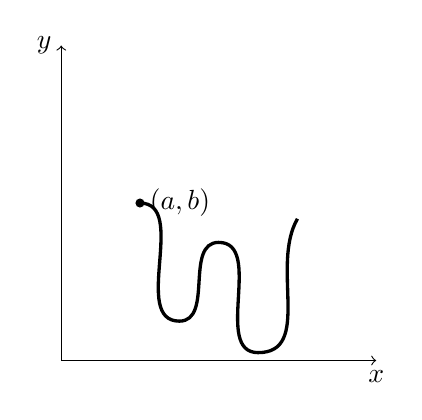
\begin{tikzpicture}
\draw[<->] (4,0) -- (0,0) -- (0,4);
\node[below] at (4,0) {$x$};
\node[left] at (0,4) {$y$};
\draw[fill] (1,2) circle [radius=0.05];
\node[right] at (1,2) {$(a,b)$};
\draw[very thick] (3,1.8) to [out=240,in=0] (2.5,0.1) to [out=180,in=0] (2,1.5) to [out=180,in=0] (1.5,0.5) to [out=180,in=0] (1,2);
\end{tikzpicture}\caption{}\label{m4}
\end{minipage}
\end{figure}

最后,可能有这样的情形,当$x$在点$a$的右方任意接近$a$时,函数$y=f(x)$的值有时大于$b$,而有时又小于$b$(图\ref{m5}). 很明显,此时当$x\to a+0$时$y$不可能是单调地趋近于其极限$b$. 此时若函数$f(x)$连续(如同我们在所有图形中所描绘的),则它必然在点$a$的右方充分靠近$a$的无穷点集上等于其极限值$b$,从几何上说,函数$f(x)$的图形在点$a$附近无限多次地穿过直线$y=b$. 

\begin{figure}[h]
\centering
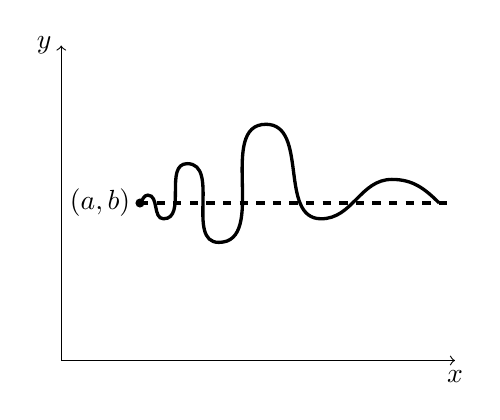
\begin{tikzpicture}
\draw[<->] (5,0) -- (0,0) -- (0,4);
\node[below] at (5,0) {$x$};
\node[left] at (0,4) {$y$};
\draw[fill] (1,2) circle [radius=0.05];
\node[left] at (1,2) {$(a,b)$};
\draw[dashed,ultra thick] (1,2) -- (5,2);
\draw[very thick] (1,2) to [out=45,in=180] (1.1,2.1) to [out=0,in=180] (1.3,1.8) to [out=0,in=180] (1.6,2.5) to [out=0,in=180] (2,1.5) to [out=0,in=180] (2.6,3) to [out=0,in=180] (3.3,1.8) to [out=0,in=180] (4.2,2.3) to [out=0,in=135] (4.8,2);
\end{tikzpicture}\caption{}\label{m5}
\end{figure}

很显然,当$x\to a+0$时趋近于$b$的连续变化的量的所有可能的类型仅限于这些情况. 我们不再去单独研究当$x\to a-0$即所有的$x$均小于$a$的情形,很明显,把图\ref{m1}至图\ref{m5}对直线$x=a$反转即可得到相应的图形. 

如果我们假设当$x\to a$时$y\to b$,则当然有$\lim_{x\to a+0} = b$以及$\lim_{x\to a-0} = b$,此时我们谈到的函数$y$当$x$从点$a$的右边的5种极限类型的每一种都可以类似地与从点$a$的左边趋近于$a$的5种类似的极限类型结合起来,从而我们就得到了当$x\to a$时函数$y\to b$的25种不同类型的极限. 

我们还要注意到,图\ref{m1}至图\ref{m4}中所描述的情形可以方便地写成相应的形式
$$
y\to b+0\; (x\to a+0)\; \textrm{及}\; y\to b-0\; (x\to a+0)\; .
$$

到目前为止,我们认定$a$及$b$是数. 当这两个字母之一(或者两个一起)表示$+\infty$或$-\infty$时,也不难列举出函数$y$的各种类型的极限. 你们自己将不难作出. 作为例子,我们指出当$a=+\infty$,而$b$是数时,所有的类型可以表示成图\ref{m1p}至图\ref{m5p}. 

\begin{figure}[h]
\begin{minipage}[b]{5cm}
\begin{tikzpicture}
\draw[<->] (4,0) -- (0,0) -- (0,4);
\node[below] at (4,0) {$x$};
\node[left] at (0,4) {$y$};
\node[below] at (2,1) {$y=b$};
\draw[dashed,ultra thick] (0,1) -- (4,1);
\draw[very thick] (0.5,2.8) to [out=140,in=180] (3.8,1.1);
\end{tikzpicture}\caption{}\label{m1p}
\end{minipage}
\hfill
\begin{minipage}[b]{5cm}
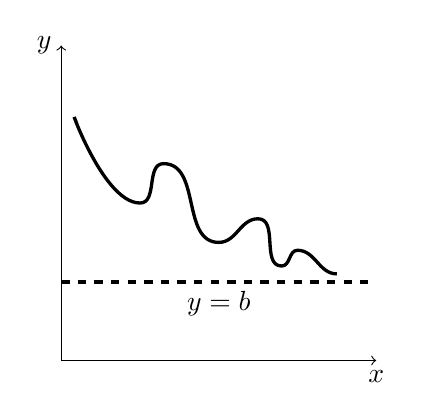
\begin{tikzpicture}
\draw[<->] (4,0) -- (0,0) -- (0,4);
\node[below] at (4,0) {$x$};
\node[left] at (0,4) {$y$};
\node[below] at (2,1) {$y=b$};
\draw[dashed,ultra thick] (0,1) -- (4,1);
\draw[very thick] (0.2,3) to [out=110,in=180] (1,2) to [out=0,in=180] (1.3,2.5) to [out=0,in=180] (2,1.5) to [out=0,in=180] (2.5,1.8) to [out=0,in=180] (2.8,1.2) to [out=0,in=180] (3,1.4) to [out=0,in=180] (3.5,1.1);
\end{tikzpicture}\caption{}\label{m2p}
\end{minipage}
\end{figure}

\begin{figure}[h]
\begin{minipage}[b]{5cm}
\begin{tikzpicture}
\draw[<->] (4,0) -- (0,0) -- (0,4);
\node[below] at (4,0) {$x$};
\node[left] at (0,4) {$y$};
\node[above] at (2,2) {$y=b$};
\draw[dashed,ultra thick] (0,2) -- (4,2);
\draw[very thick] (0.5,0.2) to [out=45,in=180] (3.8,1.9);
\end{tikzpicture}\caption{}\label{m3p}
\end{minipage}
\hfill
\begin{minipage}[b]{5cm}
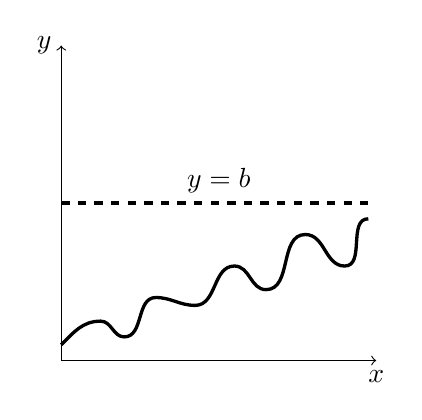
\begin{tikzpicture}
\draw[<->] (4,0) -- (0,0) -- (0,4);
\node[below] at (4,0) {$x$};
\node[left] at (0,4) {$y$};
\node[above] at (2,2) {$y=b$};
\draw[dashed,ultra thick] (0,2) -- (4,2);
\draw[very thick] (0,0.2) to [out=45,in=180] (0.5,0.5) to [out=0,in=180] (0.8,0.3) to [out=0,in=180] (1.2,0.8) to [out=0,in=180] (1.7,0.7) to [out=0, in=180] (2.2,1.2) to [out=0, in=180] (2.6,0.9) to [out=0, in=180] (3.1,1.6) to [out=0, in=180] (3.6,1.2) to [out=0, in=180] (3.9,1.8);
\end{tikzpicture}\caption{}\label{m4p}
\end{minipage}
\end{figure}

\begin{figure}[h]
\centering
\begin{minipage}[b]{4cm}
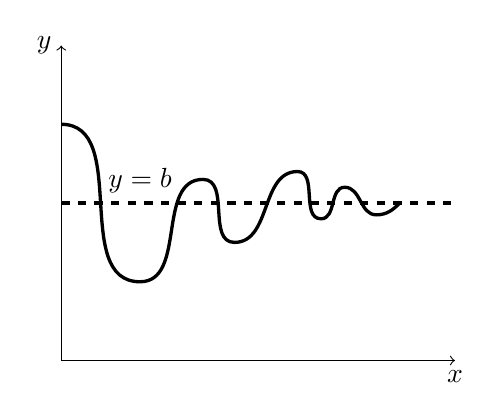
\begin{tikzpicture}
\draw[<->] (5,0) -- (0,0) -- (0,4);
\node[below] at (5,0) {$x$};
\node[left] at (0,4) {$y$};
\node[above] at (1,2) {$y=b$};
\draw[dashed,ultra thick] (0,2) -- (5,2);
\draw[very thick] (0,3) to [out=0, in=180] (1,1) to [out=0, in=180] (1.8,2.3) to [out=0, in=180] (2.2,1.5) to [out=0, in=180] (3, 2.4) to [out=0, in=180] (3.3,1.8) to [out=0, in=180] (3.6,2.2) to [out=0, in=180] (4,1.85) to [out=0, in=225] (4.3,2);
\end{tikzpicture}\caption{}\label{m5p}
\end{minipage}
\end{figure}

函数$f(x)$在图\ref{m1p}及图\ref{m3p}的情形是单调的,而在其他情形则是不单调的. 在图\ref{m5p}的情形(如果它连续的话)函数$f(x)$可以无穷多次地等于其极限值$b$(对充分大的$x$值). 

当$a$是数,而$b=+\infty$,而当$x\to a+0$时,很显然,只可能是图\ref{m6}及图\ref{m7}所描述的两种类型. 

\begin{figure}[h]
\begin{minipage}[b]{5cm}
\begin{tikzpicture}
\draw[<->] (4,0) -- (0,0) -- (0,4);
\node[below] at (4,0) {$x$};
\node[left] at (0,4) {$y$};
\node[below] at (2,0) {$a$};
\draw[dashed,ultra thick] (1,0) -- (1,4);
\draw[very thick] (1.2,3.5) to [out=270,in=180] (3.8,0.5);
\end{tikzpicture}\caption{}\label{m6}
\end{minipage}
\hfill
\begin{minipage}[b]{5cm}
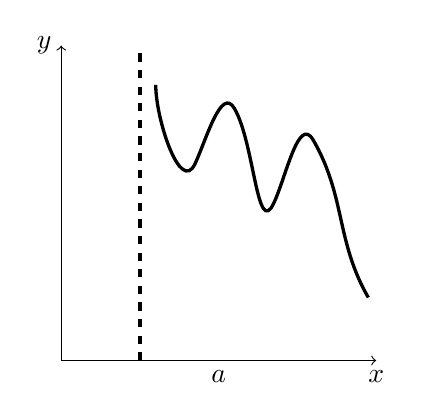
\begin{tikzpicture}
\draw[<->] (4,0) -- (0,0) -- (0,4);
\node[below] at (4,0) {$x$};
\node[left] at (0,4) {$y$};
\node[below] at (2,0) {$a$};
\draw[dashed,ultra thick] (1,0) -- (1,4);
\draw[very thick] (1.2,3.5) to [out=270,in=245] (1.7,2.5) to [out=65,in=120] (2.2,3.2) to [out=300,in=245] (2.7,2) to [out=65,in=120] (3.2,2.8) to [out=300,in=120] (3.9,0.8);
\end{tikzpicture}\caption{}\label{m7}
\end{minipage}
\end{figure}

\section{常量的极限}

当然,你们知道,常量(即仅可能取唯一的值的量)的极限总是存在的并且就等于这个唯一的值. 这个规定有时被当作不可理解的,因为我们一开始说的是变量的极限,那么怎么可以有常量的极限存在呢?

但是这个规定对我们而言,首先在逻辑上是必然的,如果我们不想在我们的极限定义中出现矛盾的话. 实际上,对任何$x$值若$y=b$,则对点$b$的无论怎样的邻域$V$,对任何$x$我们都有关系式$y\in V$,由此依照极限的定义,我们一定可以得出:对任何$a$,都有
\begin{equation}\label{funclimit}
	\lim_{x\to a} y=b\; .
\end{equation}

再其次,这个约定又是十分合理的(实际上,也几乎是不可避免的)和实用的. 事实上,如果我们暂时认为常量没有极限,而设有一个函数使(\ref{funclimit})对它成立,则大家知道
$$
\lim_{x\to a}(-y)=-b\; .
$$

但对任何$x$, $y+(-y)=0$,于是量$y$与$-y$都是有极限的,而它们的和是常量$0$,而按照我们的约定,又是没有极限的,这样一来,在表述我们熟知的两个变量和的极限的定理时,我们不得不预先声明:``只要这个和不是常量时'',和的极限的定理才成立. 类似这样附加的话,其人为的繁琐的特征是显而易见的,而我们又不得不把它们放入所有关于极限的定理之中,但若对任何常量都给以极限,我们就可以完全解脱了. 而由于,像我们已经看到的那样,我们又没有作出与我们已建立的极限概念的定义有矛盾的任何差错,所以在讲述数学分析基础时始终采用了这个约定. 

\section{无穷小和无穷大}

如果当$x\to a$时$y\to 0$,量$y=f(x)$就称为当$x\to a$时的无穷小量. 在数学分析的许多讲法中无穷小概念在极限论中都起着基本的作用,先给出它的定义,然后再给出一般的极限概念. 与此相反,一些现代学者在阐述分析教程时则完全不理会无穷小的概念,认定这个概念是多余的,它会留下,并且事实上确实是留下了许多误解. 

关于这一点应当指出,这里所谈的当然不是趋近于零的量的\CJKunderwave{概念}(这个概念在数学分析的任何讲法中,包含在其所有的应用中都起着本质的作用),而仅只是谈要不要有``无穷小量''这个\CJKunderwave{术语}. 这个名称实际上常是不通顺的并且常常导致误解,使用这个名称似乎是想去刻画这一类的量的\CJKunderwave{大小}——把一些在其变化的已知阶段完全是并不小的量,叫做无穷小量总是不方便的. 而在事实上这个名称所要描述的仅只是已知量的\CJKunderwave{变化特征},而绝不是它的大小. 这个用词上的失误应归咎于历史的遗留:无穷小量的叫法出现在这样的时代,那时这个概念的意义完全不同于我们现在为它确定的意义. 

但是,如同我们已经指明的那样,趋近于零的量在分析中以及其应用中如此经常遇到,所以拒绝给它一个简单的名词也是非常困难的. 另一方面,把在历史上已经使用了几个世纪的名称换成另外的说法确实是一场灾难,而这样的灾难在数学中总是经常不断地感觉到又毫无好处. 最后,如果我们不把无穷小量作为极限理论的基础(如同我们现在所做的那样),而仅仅是把它理解为趋于极限的量的一般概念的一种特殊情形,则概念间严重混淆的危险性就不会太大并且不致引起太严重的后果. 

量$y$称为\CJKunderwave{无穷大量},如果
$$
\lim_{x\to a}\abs{y} = +\infty\; ,
$$
这就是说,无穷大量就是要么趋于$+\infty$,要么趋于$-\infty$,要么不趋近于某个极限,而是时而取正值,时而取负值,但按其绝对值则无限增加. 这后一种情形的例子如变量$y=(-1)^n n$当$n\to +\infty$时即是,其中$n$在增加时仅取整数值. 关于术语``无穷大量''也可以重复我们上面对``无穷小量''所说的那一些话. 

这里我们毋需对我们已熟知的无穷小量的和、差、积的定理再说什么,我们只需要对常导致误解的两个地方加以注意:

1)在无穷小量的和及积的定理中经常要求加项(或因子)的个数是有限的,没有这个说明,我们容易找出简单例子来证明,这两个定理是不能成立的. 

2)关于两个无穷小量的商不可能作出任何一般的结论,这里商可以具有任何变化特征,特别地,可能不趋于任何极限. 

在继续讲解之前,我们需要对记号$+\infty$和$-\infty$再作些说明. 这些记号我们现在已经是经常遇到的了. 当然,你们知道,这些记号并不表示任何数. 例如:在问到记号$+\infty$表示什么时,最正确最清楚的就是说它本身什么意义也没有;但``$+\infty$的邻域''这种说法是有意义的,它表示的是全部大于某个(任意的)数$a$的全体实数这样一个集合;对于这样的集合给一个简单的名称是很方便的,因为在分析中,我们每每要碰到这类集合,所以就称它为$+\infty$的邻域. 与``$+\infty$的邻域''这种说法一样,诸如$\lim_{x\to a}y = +\infty$(其中$a$本身可以是符号$+\infty$与$-\infty$之一)这种表达式也就有了意义. 实际上,在我们已给出的极限定义$\lim_{x\to a}y = b$中谈到的字母$a$及$b$时总是与它们的邻域一起谈到的. 因此,这两个字母中任何一个都可以符号$+\infty$(或者$-\infty$)来代替(只要我们指明,把什么样的集合称之为这些符号的邻域就行),没有必要对这些符号本身给予任何意义. 

从所有这些可以明白,在使用符号$+\infty$及$-\infty$时该要多么细心. 特别地,对它们作某些算术运算($\frac{1}{\infty} = 0$等等)是完全不能允许的,而在某些``简略''的分析教程中是这样用的. 同样地,所有其式中有符号$+\infty$及$-\infty$出现的等式,如果这些符号虽不是直接起着上述类型的极限的作用,也都是没有意义的. 如三角表示中形如$\tan{\frac{\pi}{2}} = \pm \infty$ \footnote{当然,正确的表述应当是$$\lim_{x\to \frac{\pi}{2}-0 }\tan{x} = +\infty\; , \lim_{x\to \frac{\pi}{2}+0} \tan{x} = -\infty\; .$$} 之类的任何等式都是如此. 反之,不等式
$$a<+\infty\; , b>-\infty\; , -\infty < c < +\infty$$
却可以有确定的意义. 它们依次表示:1)$a$要么是一个数,要么是符号$-\infty$; 2)$b$要么是一个数,要么是符号$+\infty$;3)$c$是一个数. 

最后,在谈到函数$y=f(x)$的极限存在时,必须准确地声明,我们这里所说的是存在一个\CJKunderwave{数},它是这个量的极限,或者我们也将允许符号$+\infty\; , -\infty$作为极限. 当然,在这里的术语问题上,我们显然可以取两种说法中的任何一个,于是乎怎样选择就应当看它是否适合. 通常约定把``$y$有极限''理解为存在着一个\CJKunderwave{数}作为量$y$的极限,如果需要对这个诊断作广义的理解,则应作专门的声明. 在今后我们都将这样处理. 

\section{Cauchy准则}

极限理论的最重要的问题之一是:已知函数$y=f(x)$,要问:当$x\to a$时它是否有极限?在此:1)按照我们的约定要讨论的是这样的数$b$的存在问题,使当$x\to a$时$y\to b$;2)反之,$a$可以是数,也可以是符号$+\infty$与$-\infty$两者之一;3)在此问题中只谈及极限的存在性问题,至于怎样去找出这里的极限,我们目前完全不必去管它. 

下述的极限存在的重要准则是十分重要的工具,特别在理论研究中是这样. 

\begin{newthem}[Cauchy准则]
要使函数$y=f(x)$当$x\to a$时有极限,必须而且只需下述条件得到满足:(A)\ 无论对于怎样小的正数$\epsilon$,都存在着数(或符号)$a$的一个这样的邻域$U$,使得对邻域$U$中的任何两个数$x_1$和$x_2$,都有$$\abs{f(x_1)-f(x_2)} < \epsilon .$$
\end{newthem}

\begin{newproof}
1) 假设当$x\to a$时,量$y$趋近于数$b$. 依照极限的定义,存在数$b$的邻域,使得$y$位于$b-\frac{\epsilon}{2}$与$b+\frac{\epsilon}{2}$之间,因而彼此之差小于$\epsilon$. 这就证明了条件(A)的必要性.

2) 现在设条件(A)成立. 对每一个自然数$n$都存在着数$a$的这样一个邻域$U_n$,使得当$x_1\in U_n$,$x_2\in U_n$时我们总有

\begin{equation}
\abs{f(x_1)-f(x_2)} < \frac{1}{n}.
\label{cauchy-condition-sequence-form}
\end{equation}

我们可以把每一个这样的邻域$U_n$都取为区间(闭的),同时我们有权假设$U_{n+1}\subset U_n(n=1,2,\cdots)$,实际上,若区间$U_{n+1}$不是区间$U_n$的一部分,则我们通常取区间$U_n$与$U_{n+1}$的公共部分$U'_{n+1}$来代替$U_{n+1}$\footnote{显然,它是非空的.}. 很明显,$U'_{n+1}$是区间,且$U'_{n+1}\subset U_n$,并且对任何$x_1\in U'_{n+1}$,$x_2\in U'_{n+1}$我们都有
$$
\abs{f(x_1)-f(x_2)} < \frac{1}{n+1},
$$
所以邻域$U'_{n+1}$在任何情况下都是可以用来代替邻域$U_{n+1}$的.

因为函数$f(x)$在区间$U_n$上是满足条件(\ref{cauchy-condition-sequence-form})的,则函数在此区间上所取的值的整个集合$M_n$将落在长度为$\frac{1}{n}$的某个区间$\Delta_n$之内:$\Delta_{n+1}\subset \Delta_n$;又因为当$n\to \infty$时区间$\Delta_n$的长度$\frac{1}{n}$将趋近于零,则区间序列$\Delta_n(n=1,2,\cdots)$将构成收缩的区间套. 根据第一讲的引理\ref{sequence_lemma_plus},我们就可以断定,存在着唯一的一个数$b$属于所有的区间$\Delta_n$.

最后,我们来证明$\lim_{x\to a}y = b$. 为此我们以$V$来表示数$b$的任意邻域. 依照这个数的定义,对任何充分大的$n$有$\Delta_n\subset V$. 所以,若$x\in U_n$,则$f(x)\in M_n \subset \Delta_n \subset V$,由此,依照极限的定义应有$\lim_{x\to a}y = b$.
\end{newproof}

这样一来,Cauchy准则就已完全证明. 特别地,要使数序列
$$
a_1, a_2, \cdots, a_n, \cdots
$$
有极限,必须而且只需:对任意的$\epsilon > 0$以及任何充分大的$n$和$m$都有
$$
\abs{a_n - a_m} < \epsilon.
$$
Cauchy准则只在证明某些个别的函数的极限存在性时,在很少有的情形下才得到具体的应用,为此常常采用更为简单的准则,但这种准则不是极限存在的特征,即不是必要充分的准则. 相反地,在一般的理论研究中,Cauchy准则正是由于这个特点,却能起到几乎是不可取代的作用,这一点我们即将看到. 

\section{关于基本定理的注记}

极限理论的基本定理,即和、差、积等极限定理,你们当然是很熟悉的,我们这里不仅不需再去证明,而且也不必去陈述它们,但与这些定理相关的一个注记我们还必须给出,因为这个注记对于整个一系列定理都是相同的,我们将只以其中的任一个为例来加以说明. 

当我们说到``两个量之和的极限等于它们的极限之和''(在大量``简略''的教程中正是使用这样简单的措辞的),因而我们这里指的是(尽管没有提到这一点):所有的3个量(两个加项以及和)都是有极限的,并且问题仅只涉及这些极限之间的关系. 实际上,我们这里假设多于所需,只需假设这两个加项每一项都存在极限就够了;因为这时可以证明两者之各必有极限(等于加项的极限之和). 对这个证明不需任何附加的讨论,这个结果可以从和的极限的定理的任何证明中自动地得出,成为一个附加的结果. 

反之,从和有极限则不能直接推出每一个加项都有极限,实际上,设量$y$当$x\to a$时不趋近于任何极限,很显然,量$1-y$也同样地没有极限,但是这两个量之和(是一个常数,$y+1-y=1$)当$x\to a$时有极限$1$.

这也就是说,关于和的极限的定理的最完整的陈述应当说成是:\CJKunderwave{如果已知的有限多个量中的每一个当$x\to a$时都有极限,则它们的和此时也有极限,并且和的极限等于各项的极限之和}. 所有这一系列的定理都有类似的陈述.

\section{部分极限,上极限和下极限}

我们现在需要来详细研究变量$x$的这样的函数,这些函数当$x\to a$时没有极限. 所有``简略''的教程通常是完全不研究这个问题的. 

如果对于数$a$的无论怎样的邻域$U$以及数$b$的无论怎样的邻域$V$,都可以找到一个异于$a$的点$x\in U$,使得$f(x)\in V$,当$x\to a$时,我们称数$b$是函数$y=f(x)$的部分极限. 这个简单的定义可以不加任何改变地推广到$b$是符号$+\infty$或$-\infty$之一的情形. 这就是说,部分极限$b$是这样的数,使得不论怎样靠近$a$,总可以找到$x$值,使相应的量$y$任意地接近于$b$【当$a$或$b$是$+\infty$时,我们当然应当把``任意接近于$a$(或$b$)''改变成``任意大的数'',当$a$或$b$是$-\infty$时也完全类似】.

相仿地,我们也可以定义当$n\to \infty$时数列$a_1,a_2,\cdots,a_n,\cdots$的部分极限. 

如果$\lim_{x\to a}y$存在,则正如我们从极限概念的定义中所直接看到的那样,它必然也是量$y$的一个部分极限(且是唯一的),而不管这个极限是一个数或是符号$+\infty$与$-\infty$两者之一. 但如果这个极限不存在,则这个量$y$至少有两个不同的部分极限. 这也就是说,任何函数$y=f(x)$当$x\to a$时都至少有一个部分极限,要使部分极限是唯一的,必须而且只需$\lim_{x\to a}y$存在. 

要证明这些论断的正确性,显然,我们必须证明两个命题:

\begin{newprop}
\label{part-lim}
任何函数$y=f(x)$当$x\to a$时都至少有一个部分极限.
\end{newprop}

\begin{newprop}
如果$b$是函数$y=f(x)$当$x\to a$时的唯一部分极限,则$\lim_{x\to a}y = b$.
\label{part-lim-2}
\end{newprop}

所有这些情形里,所有的极限和部分极限都可以是数,也可以是符号$+\infty$及$-\infty$.

\begin{newproof}[第一个命题]
若符号$+\infty$与$-\infty$之一是量$y$的当$x\to a$时的部分极限,则命题已经得证,因此我们假设这里不是这样,并且指明这时存在着一个数$b$,它是量$y$当$x\to a$时的部分极限. 

但若无论$+\infty$或者$-\infty$都不是函数$f(x)$当$x\to a$时的部分极限的话,则很显然,存在着这样的一对数$\alpha,\beta (\alpha < \beta)$,使得对任何充分靠近$a$的$x$,都有$$\alpha \leqslant f(x) \leqslant \beta.$$

特别地,这就表明:\CJKunderwave{在数$a$的任何邻域内都可以找到这样的数$x$,使得}$f(x)$属于区间$[\alpha, \beta]$,这样的区间为简便计,我们表之以$\Delta_1$,我们约定只用$\mathcal{A}$这个字母来表示区间$\Delta_1$所具有的以上所陈述的性质. 如果我们将此区间等分,则其两个半区间中至少有一个具有性质$\mathcal{A}$(因为若数$a$的邻域$U_1$不含任何使得$f(x)$属于左半区间$\Delta_1$的$x$,而邻域$U_2$则不含任何使$f(x)$属于其右区间的$x$的话,则作为这两个部分$U_1$与$U_2$的公共部分所组成的邻域$U$\footnote{译者注:$U = U_1 \cap U_2$}很显然将不包含任何使$f(x) \in \Delta_1$的点$x$,即区间$\Delta_t$不具有性质$\mathcal{A}$. 我们再用$\Delta_2$来表示区间$\Delta_1$的具有性质$\mathcal{A}$的一半,并且重复进行我们对区间$\Delta_1$所进行的工作即把它平分且把具有性质$\mathcal{A}$的一半表之以$\Delta_3$. 无限继续这个过程,很显然,我们就得到一个收缩的区间套$\Delta_1, \Delta_2, \Delta_3, \cdots, \Delta_n, \cdots$. 设$b$就是根据收缩区间套引理而一定存在的属于所有这些区间的唯一的公共的数,并以$U$和$V$来表示数$a$及$b$的相应的邻域. 依照数$b$的定义,可以找到一个区间$\Delta_n \subset V$,但每一个区间$\Delta_n$都具有性质$\mathcal{A}$,因而存在着这样的一个数$x\in U$,使得$f(x)\in \Delta_n \subset V$. 但此即表明,$b$是量$y$当$x\to a$时的部分极限.
\end{newproof}

\end{document}
